\documentclass[11pt,letterpaper]{article}
\usepackage[lmargin=1in,rmargin=1in,tmargin=1in,bmargin=1in]{geometry}
\usepackage{../style/homework}
\usepackage{../style/commands}
\setbool{quotetype}{false} % True: Side; False: Under
\setbool{hideans}{false} % Student: True; Instructor: False

% -------------------
% Content
% -------------------
\begin{document}

\homework{8: Due 01/14}{Do I need to be liked? Absolutely not. I like to be liked. I enjoy being liked. I have to be liked, but it's not like this compulsive need to be liked, like my need to be praised.}{Michael Scott, The Office}

% Problem 1
\problem{10} Showing all your work, factor $x^2 + 23x + 120$. \pspace

\sol 
	\begin{table}[!ht]
	\centering
	\underline{\bfseries 120} \pvspace{0.2cm}
	\begin{tabular}{rr}
	$1 \cdot 120$ & $121$ \\
	$-1 \cdot -120$ & $-121$ \\
	$2 \cdot 60$ & $62$ \\
	$-2 \cdot -60$ & $-62$ \\
	$3 \cdot 40$ & $43$ \\
	$-3 \cdot -40$ & $-43$ \\
	$4 \cdot 30$ & $34$ \\
	$-4 \cdot -30$ & $-34$ \\
	$5 \cdot 24$ & $29$ \\
	$-5 \cdot -24$ & $-29$ \\
	$6 \cdot 20$ & $26$ \\
	$-6 \cdot -20$ & $-26$ \\ \hline
	\multicolumn{1}{|r}{$8 \cdot 15$} & \multicolumn{1}{r|}{$23$} \\ \hline
	$-8 \cdot -15$ & $-23$ \\
	$10 \cdot 12$ & $22$ \\
	$-10 \cdot -12$ & $-22$ \\
	\end{tabular}
	\end{table}

Therefore,
	\[
	x^2 + 23x + 120= (x + 8)(x + 15)
	\]



\newpage



% Problem 2
\problem{10} Showing all your work, factor $-x^2 - 6x + 72$. \pspace

\sol First, we rewrite this as $-(x^2 + 6x - 72)$. Then\dots
	\begin{table}[!ht]
	\centering
	\underline{\bfseries 56} \pvspace{0.2cm}
	\begin{tabular}{rr}
	$1 \cdot -72$ & $-71$ \\
	$-1 \cdot 72$ & $71$ \\
	$2 \cdot -36$ & $-34$ \\
	$-2 \cdot 36$ & $34$ \\
	$3 \cdot -26$ & $-23$ \\
	$-3 \cdot 26$ & $23$ \\
	$4 \cdot -18$ & $-14$ \\
	$-4 \cdot 18$ & $14$ \\
	$6 \cdot -12$ & $-6$ \\ \hline
	\multicolumn{1}{|r}{$-6 \cdot 12$} & \multicolumn{1}{r|}{$6$} \\ \hline
	$8 \cdot -9$ & $-1$ \\
	$-8 \cdot 9$ & $1$ \\	
	\end{tabular}
	\end{table}

Therefore,
	\[
	-x^2 - 6x + 72= -(x^2 + 6x - 72)= -(x - 6)(x + 12)
	\]



\newpage



% Problem 3
\problem{10} Showing all your work, factor $18x^2 + 67x - 20$. \pspace

\sol 
	\begin{table}[!ht]
	\centering
	\underline{\bfseries 20} \pvspace{0.1cm}
	\begin{tabular}{c}
	$1 \cdot -20$ \\
	$-1 \cdot 20$ \\
	$2 \cdot -10$ \\
	$-2 \cdot 10$ \\
	$4 \cdot -5$ \\
	$-4 \cdot 5$
	\end{tabular}
	\end{table}

Then as $18= 1 \cdot 18= 2 \cdot 9= 3 \cdot 6$, we have\dots
	\[
	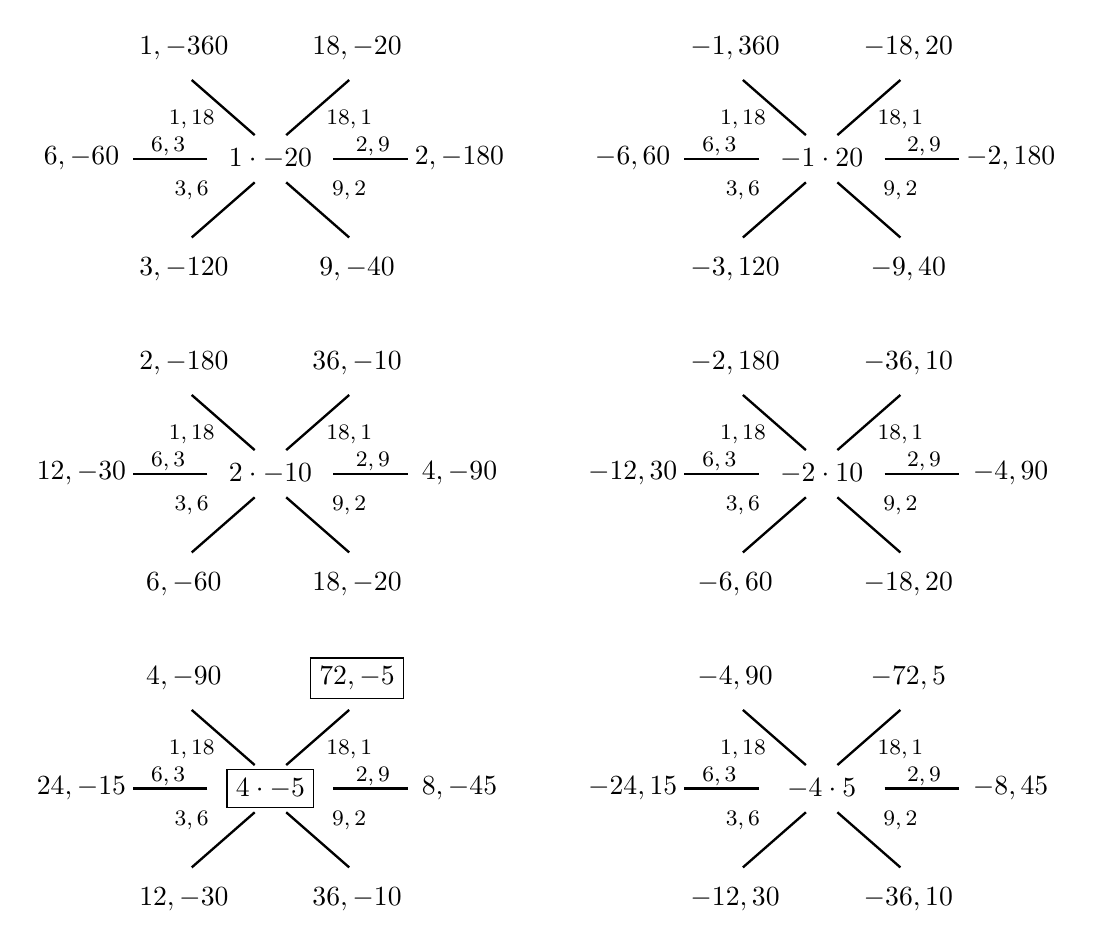
\begin{tikzpicture}
	\node at (0,0) {$1 \cdot -20$};
	\node at (-1.0,0.5) {\footnotesize$1, 18$};
	\draw[line width=0.03cm,label={1}] (-0.2,0.3) -- (-1,1);
	\node at (-1.1,1.4) {$1, -360$};
	\node at (1.0,0.5) {\footnotesize$18, 1$};
	\draw[line width=0.03cm] (0.2,0.3) -- (1,1);	
	\node at (1.1,1.4) {$18, -20$};	
	\node at (1.3,0.15) {\footnotesize$2, 9$};
	\draw[line width=0.03cm] (0.8,0) -- (1.75,0);
	\node at (2.4,0) {$2, -180$};
	\node at (1.0,-0.4) {\footnotesize$9, 2$};
	\draw[line width=0.03cm] (0.2,-0.3) -- (1,-1);
	\node at (1.1,-1.4) {$9, -40$};
	\node at (-1.0,-0.4) {\footnotesize$3, 6$};
	\draw[line width=0.03cm,label={1}] (-0.2,-0.3) -- (-1,-1);
	\node at (-1.1,-1.4) {$3, -120$};
	\node at (-1.3,0.15) {\footnotesize$6, 3$};
	\draw[line width=0.03cm] (-0.8,0) -- (-1.75,0);
	\node at (-2.4,0) {$6, -60$};
	
	\tikzset{shift={(7,0)}}

	\node at (0,0) {$-1 \cdot 20$};
	\node at (-1.0,0.5) {\footnotesize$1, 18$};
	\draw[line width=0.03cm,label={1}] (-0.2,0.3) -- (-1,1);
	\node at (-1.1,1.4) {$-1, 360$};
	\node at (1.0,0.5) {\footnotesize$18, 1$};
	\draw[line width=0.03cm] (0.2,0.3) -- (1,1);	
	\node at (1.1,1.4) {$-18, 20$};	
	\node at (1.3,0.15) {\footnotesize$2, 9$};
	\draw[line width=0.03cm] (0.8,0) -- (1.75,0);
	\node at (2.4,0) {$-2, 180$};
	\node at (1.0,-0.4) {\footnotesize$9, 2$};
	\draw[line width=0.03cm] (0.2,-0.3) -- (1,-1);
	\node at (1.1,-1.4) {$-9, 40$};
	\node at (-1.0,-0.4) {\footnotesize$3, 6$};
	\draw[line width=0.03cm,label={1}] (-0.2,-0.3) -- (-1,-1);
	\node at (-1.1,-1.4) {$-3, 120$};
	\node at (-1.3,0.15) {\footnotesize$6, 3$};
	\draw[line width=0.03cm] (-0.8,0) -- (-1.75,0);
	\node at (-2.4,0) {$-6, 60$};

	\tikzset{shift={(-7,-4)}}

	\node at (0,0) {$2 \cdot -10$};
	\node at (-1.0,0.5) {\footnotesize$1, 18$};
	\draw[line width=0.03cm,label={1}] (-0.2,0.3) -- (-1,1);
	\node at (-1.1,1.4) {$2, -180$};
	\node at (1.0,0.5) {\footnotesize$18, 1$};
	\draw[line width=0.03cm] (0.2,0.3) -- (1,1);	
	\node at (1.1,1.4) {$36, -10$};	
	\node at (1.3,0.15) {\footnotesize$2, 9$};
	\draw[line width=0.03cm] (0.8,0) -- (1.75,0);
	\node at (2.4,0) {$4, -90$};
	\node at (1.0,-0.4) {\footnotesize$9, 2$};
	\draw[line width=0.03cm] (0.2,-0.3) -- (1,-1);
	\node at (1.1,-1.4) {$18, -20$};
	\node at (-1.0,-0.4) {\footnotesize$3, 6$};
	\draw[line width=0.03cm,label={1}] (-0.2,-0.3) -- (-1,-1);
	\node at (-1.1,-1.4) {$6, -60$};
	\node at (-1.3,0.15) {\footnotesize$6, 3$};
	\draw[line width=0.03cm] (-0.8,0) -- (-1.75,0);
	\node at (-2.4,0) {$12, -30$};

	\tikzset{shift={(7,0)}}

	\node at (0,0) {$-2 \cdot 10$};
	\node at (-1.0,0.5) {\footnotesize$1, 18$};
	\draw[line width=0.03cm,label={1}] (-0.2,0.3) -- (-1,1);
	\node at (-1.1,1.4) {$-2, 180$};
	\node at (1.0,0.5) {\footnotesize$18, 1$};
	\draw[line width=0.03cm] (0.2,0.3) -- (1,1);	
	\node at (1.1,1.4) {$-36, 10$};	
	\node at (1.3,0.15) {\footnotesize$2, 9$};
	\draw[line width=0.03cm] (0.8,0) -- (1.75,0);
	\node at (2.4,0) {$-4, 90$};
	\node at (1.0,-0.4) {\footnotesize$9, 2$};
	\draw[line width=0.03cm] (0.2,-0.3) -- (1,-1);
	\node at (1.1,-1.4) {$-18, 20$};
	\node at (-1.0,-0.4) {\footnotesize$3, 6$};
	\draw[line width=0.03cm,label={1}] (-0.2,-0.3) -- (-1,-1);
	\node at (-1.1,-1.4) {$-6, 60$};
	\node at (-1.3,0.15) {\footnotesize$6, 3$};
	\draw[line width=0.03cm] (-0.8,0) -- (-1.75,0);
	\node at (-2.4,0) {$-12, 30$};
	
	\tikzset{shift={(-7,-4)}}

	\node at (0,0) {\framebox{$4 \cdot -5$}};
	\node at (-1.0,0.5) {\footnotesize$1, 18$};
	\draw[line width=0.03cm,label={1}] (-0.2,0.3) -- (-1,1);
	\node at (-1.1,1.4) {$4, -90$};
	\node at (1.0,0.5) {\footnotesize$18, 1$};
	\draw[line width=0.03cm] (0.2,0.3) -- (1,1);	
	\node at (1.1,1.4) {\framebox{$72, -5$}};	
	\node at (1.3,0.15) {\footnotesize$2, 9$};
	\draw[line width=0.03cm] (0.8,0) -- (1.75,0);
	\node at (2.4,0) {$8, -45$};
	\node at (1.0,-0.4) {\footnotesize$9, 2$};
	\draw[line width=0.03cm] (0.2,-0.3) -- (1,-1);
	\node at (1.1,-1.4) {$36, -10$};
	\node at (-1.0,-0.4) {\footnotesize$3, 6$};
	\draw[line width=0.03cm,label={1}] (-0.2,-0.3) -- (-1,-1);
	\node at (-1.1,-1.4) {$12, -30$};
	\node at (-1.3,0.15) {\footnotesize$6, 3$};
	\draw[line width=0.03cm] (-0.8,0) -- (-1.75,0);
	\node at (-2.4,0) {$24, -15$};

	\tikzset{shift={(7,0)}}

	\node at (0,0) {$-4 \cdot 5$};
	\node at (-1.0,0.5) {\footnotesize$1, 18$};
	\draw[line width=0.03cm,label={1}] (-0.2,0.3) -- (-1,1);
	\node at (-1.1,1.4) {$-4, 90$};
	\node at (1.0,0.5) {\footnotesize$18, 1$};
	\draw[line width=0.03cm] (0.2,0.3) -- (1,1);	
	\node at (1.1,1.4) {$-72, 5$};	
	\node at (1.3,0.15) {\footnotesize$2, 9$};
	\draw[line width=0.03cm] (0.8,0) -- (1.75,0);
	\node at (2.4,0) {$-8, 45$};
	\node at (1.0,-0.4) {\footnotesize$9, 2$};
	\draw[line width=0.03cm] (0.2,-0.3) -- (1,-1);
	\node at (1.1,-1.4) {$-36, 10$};
	\node at (-1.0,-0.4) {\footnotesize$3, 6$};
	\draw[line width=0.03cm,label={1}] (-0.2,-0.3) -- (-1,-1);
	\node at (-1.1,-1.4) {$-12, 30$};
	\node at (-1.3,0.15) {\footnotesize$6, 3$};
	\draw[line width=0.03cm] (-0.8,0) -- (-1.75,0);
	\node at (-2.4,0) {$-24, 15$};
	\end{tikzpicture}
	\] \pspace

Therefore, 
	\[
	18x^2 + 67x - 20= (18x - 5)(x + 4)
	\]



\newpage



% Problem 4
\problem{10} Use the quadratic equation to factor $100x^2 - 225x + 126$. \pspace

\sol We have\dots \pspace
	\[
	\begin{aligned}
	x&= \dfrac{-b \pm \sqrt{b^2 - 4ac}}{2a} \\[0.3cm]
	x&= \dfrac{-(-225) \pm \sqrt{(-225)^2 - 4(100)(126)}}{2(100)} \\[0.3cm]
	x&= \dfrac{225 \pm \sqrt{50625 - 50400}}{200} \\[0.3cm]
	x&= \dfrac{225 \pm \sqrt{225}}{200} \\[0.3cm]
	x&= \dfrac{225 \pm 15}{200}
	\end{aligned}
	\] \pspace
But then the roots of $100x^2 - 225x + 126$ are $x= \frac{225 + 15}{200}= \frac{240}{200}= \frac{6}{5}$ or $x= \frac{225 - 15}{200}= \frac{21}{20}$. Observe that $a= 1$. Therefore, the factorization is\dots
	\[
	100x^2 - 225x + 126= 100 \cdot \left(x - \dfrac{6}{5} \right) \left(x - \dfrac{21}{20} \right)= 5 \cdot \left(x - \dfrac{6}{5} \right) \cdot 20\left(x - \dfrac{21}{20} \right)= (5x - 6)(20x - 21)
	\]



\newpage



% Problem 5
\problem{10} Use the quadratic equation to factor $x^2 - 6x + 1$. \pspace

\sol We have\dots \pspace
	\[
	\begin{aligned}
	x&= \dfrac{-b \pm \sqrt{b^2 - 4ac}}{2a} \\[0.3cm]
	x&= \dfrac{-(-6) \pm \sqrt{(-6)^2 - 4(1)(1)}}{2(1)} \\[0.3cm]
	x&= \dfrac{6 \pm \sqrt{36 - 4}}{2} \\[0.3cm]
	x&= \dfrac{6 \pm \sqrt{32}}{2} \\[0.3cm]
	x&= \dfrac{6 \pm \sqrt{16 \cdot 2}}{2} \\[0.3cm]
	x&= \dfrac{6 \pm 4\sqrt{2}}{2} \\[0.3cm]
	x&= 3 \pm 2 \sqrt{2}
	\end{aligned}
	\] \pspace
Then the roots of $x^2 - 6x + 1$ are $x= 3 + 2\sqrt{2}$ and $x= 3 - 2\sqrt{2}$. Observe that $a= 1$. Therefore, the factorization is\dots \pspace
	\[
	x^2 - 6x + 1= 1 \cdot \big(x - (3 + 2\sqrt{2}) \big) \big(x - (3 - 2\sqrt{2}) \big)= \big(x - (3 + 2\sqrt{2}) \big) \big(x - (3 - 2\sqrt{2}) \big)
	\]



\newpage



% Problem 6
\problem{10} Showing all your work, solve the equation $x^2 - 9x + 14= 0$. \pspace

\sol
	\[
	\begin{aligned}
	x^2 - 9x + 14&= 0 \\[0.3cm]
	(x - 2)(x - 7)&= 0
	\end{aligned}
	\] \pspace
But then either $x - 2=0$, which implies $x= 2$, or $x - 7= 0$, which implies $x= 7$. Therefore, $x= 2$ or $x= 7$. 



\newpage



% Problem 7
\problem{10} Showing all your work, solve the equation $x^2 + 2x= 48$. \pspace

\sol We have\dots \pspace
	\[
	\begin{aligned}
	x^2 + 2x&= 48 \\[0.3cm]
	x^2 + 2x - 48&= 0 \\[0.3cm]
	(x + 8)(x - 6)&= 0 
	\end{aligned}
	\] \pspace
But then either $x + 8= 0$, which implies $x= -8$, or $x - 6= 0$, which implies $x= 6$. Therefore, $x= -8$ or $x= 6$. 



\newpage



% Problem 8
\problem{10} Showing all your work, solve the equation $x= 15 - 2x^2$. \pspace

\sol We have\dots \pspace
	\[
	\begin{aligned}
	x= 15 &- 2x^2 \\[0.3cm]
	2x^2 + x - 15&= 0 \\[0.3cm]
	(2x - 5)(x + 3)&= 0 
	\end{aligned}
	\] \pspace
But then either $2x - 5= 0$, which implies that $2x= 5$ so that $x= \frac{5}{2}$, or $x + 3= 0$, which implies that $x= -3$. Therefore, $x= -3$ or $x= \frac{5}{2}$. 



\newpage



% Problem 9
\problem{10} Use the quadratic equation to solve the equation $x^2= 2x + 13$. \pspace

\sol First, we write the equation as\dots
	\[
	\begin{aligned}
	x^2= 2x &+ 13 \\
	x^2 - 2x - 13&= 0
	\end{aligned}
	\]
Then we have\dots \pspace
	\[
	\begin{aligned}
	x&= \dfrac{-b \pm \sqrt{b^2 - 4ac}}{2a} \\[0.3cm]
	x&= \dfrac{-(-2) \pm \sqrt{(-2)^2 - 4(1)(-13)}}{2(1)} \\[0.3cm]
	x&= \dfrac{2 \pm \sqrt{4 + 52}}{2} \\[0.3cm]
	x&= \dfrac{2 \pm \sqrt{56}}{2} \\[0.3cm]
	x&= \dfrac{2 \pm \sqrt{4 \cdot 14}}{2} \\[0.3cm]
	x&= \dfrac{2 \pm 2\sqrt{14}}{2} \\[0.3cm]
	x&= 1 \pm \sqrt{14}
	\end{aligned}
	\] \pspace
Then either $x= 1 + \sqrt{14}$ or $x= 1 - \sqrt{14}$. Therefore, $x= 1 - \sqrt{14}, 1 + \sqrt{14}$. 



\newpage



% Problem 10
\problem{10} Use the quadratic equation to solve the equation $x^2 + 29= 10x$. \pspace

\sol First, we write the equation as\dots
	\[
	\begin{aligned}
	x^2 + 29&= 10x \\
	x^2 - 10x + 29&= 0 
	\end{aligned}
	\]
Then we have\dots \pspace
	\[
	\begin{aligned}
	x&= \dfrac{-b \pm \sqrt{b^2 - 4ac}}{2a} \\[0.3cm]
	x&= \dfrac{-(-10) \pm \sqrt{(-10)^2 - 4(1)(29)}}{2(1)} \\[0.3cm]
	x&= \dfrac{10 \pm \sqrt{100 - 116}}{2} \\[0.3cm]
	x&= \dfrac{10 \pm \sqrt{-16}}{2} \\[0.3cm]
	x&= \dfrac{10 \pm \sqrt{16}i}{2} \\[0.3cm]
	x&= \dfrac{10 \pm 4i}{2} \\[0.3cm]
	x&= 5 \pm 2i
	\end{aligned}
	\] \pspace
Then $x= 5 + 2i$ or $x= 5 - 2i$. Therefore, $x= 5 - 2i, 5 + 2i$. 


\end{document}